% --------------------------------------------------------------
% This is all preamble stuff that you don't have to worry about.
% Head down to where it says "Start here"
% --------------------------------------------------------------
 
\documentclass[12pt]{article}

\usepackage[margin=1in]{geometry}
\usepackage{color}
\setlength{\headsep}{0.75 in}
\setlength{\parindent}{0 in}
\setlength{\parskip}{0.1 in}
 
\usepackage[margin=1in]{geometry} 
\usepackage{amsmath,amsthm,amssymb}
\usepackage{graphicx}
\usepackage{subfig}
\usepackage{float}
\graphicspath{ {images/} }

\addtolength{\topmargin}{-0.5in}

 
\newcommand{\N}{\mathbb{N}}
\newcommand{\Z}{\mathbb{Z}}
 
\newenvironment{theorem}[2][Theorem]{\begin{trivlist}
\item[\hskip \labelsep {\bfseries #1}\hskip \labelsep {\bfseries #2.}]}{\end{trivlist}}
\newenvironment{lemma}[2][Lemma]{\begin{trivlist}
\item[\hskip \labelsep {\bfseries #1}\hskip \labelsep {\bfseries #2.}]}{\end{trivlist}}
\newenvironment{exercise}[2][Exercise]{\begin{trivlist}
\item[\hskip \labelsep {\bfseries #1}\hskip \labelsep {\bfseries #2.}]}{\end{trivlist}}
\newenvironment{problem}[2][Problem]{\begin{trivlist}
\item[\hskip \labelsep {\bfseries #1}\hskip \labelsep {\bfseries #2.}]}{\end{trivlist}}
\newenvironment{question}[2][Question]{\begin{trivlist}
\item[\hskip \labelsep {\bfseries #1}\hskip \labelsep {\bfseries #2.}]}{\end{trivlist}}
\newenvironment{corollary}[2][Corollary]{\begin{trivlist}
\item[\hskip \labelsep {\bfseries #1}\hskip \labelsep {\bfseries #2.}]}{\end{trivlist}}
 
\begin{document}
 
% --------------------------------------------------------------
%                         Start here
% --------------------------------------------------------------

\title{\textbf{A4: \\ Photoplethysmography}}%replace X with the appropriate number
\author{\textbf{Group 5}\\ %replace with your name
Thai Nguyen, Gahyun (Susie) Kim, \\ Colin Stern} %if necessary, replace with your course title
\vspace{-10mm}
\maketitle
 
 

\begin{enumerate}

% --------------------------------------------------------------
%                         PPG Signal
% --------------------------------------------------------------
\item \textbf{Smoothed and Unsmoothed PPG Signal Displayed on Android UI}

\begin{figure}[!htb]
  \centering
  \subfloat[Smoothed PPG Signal]{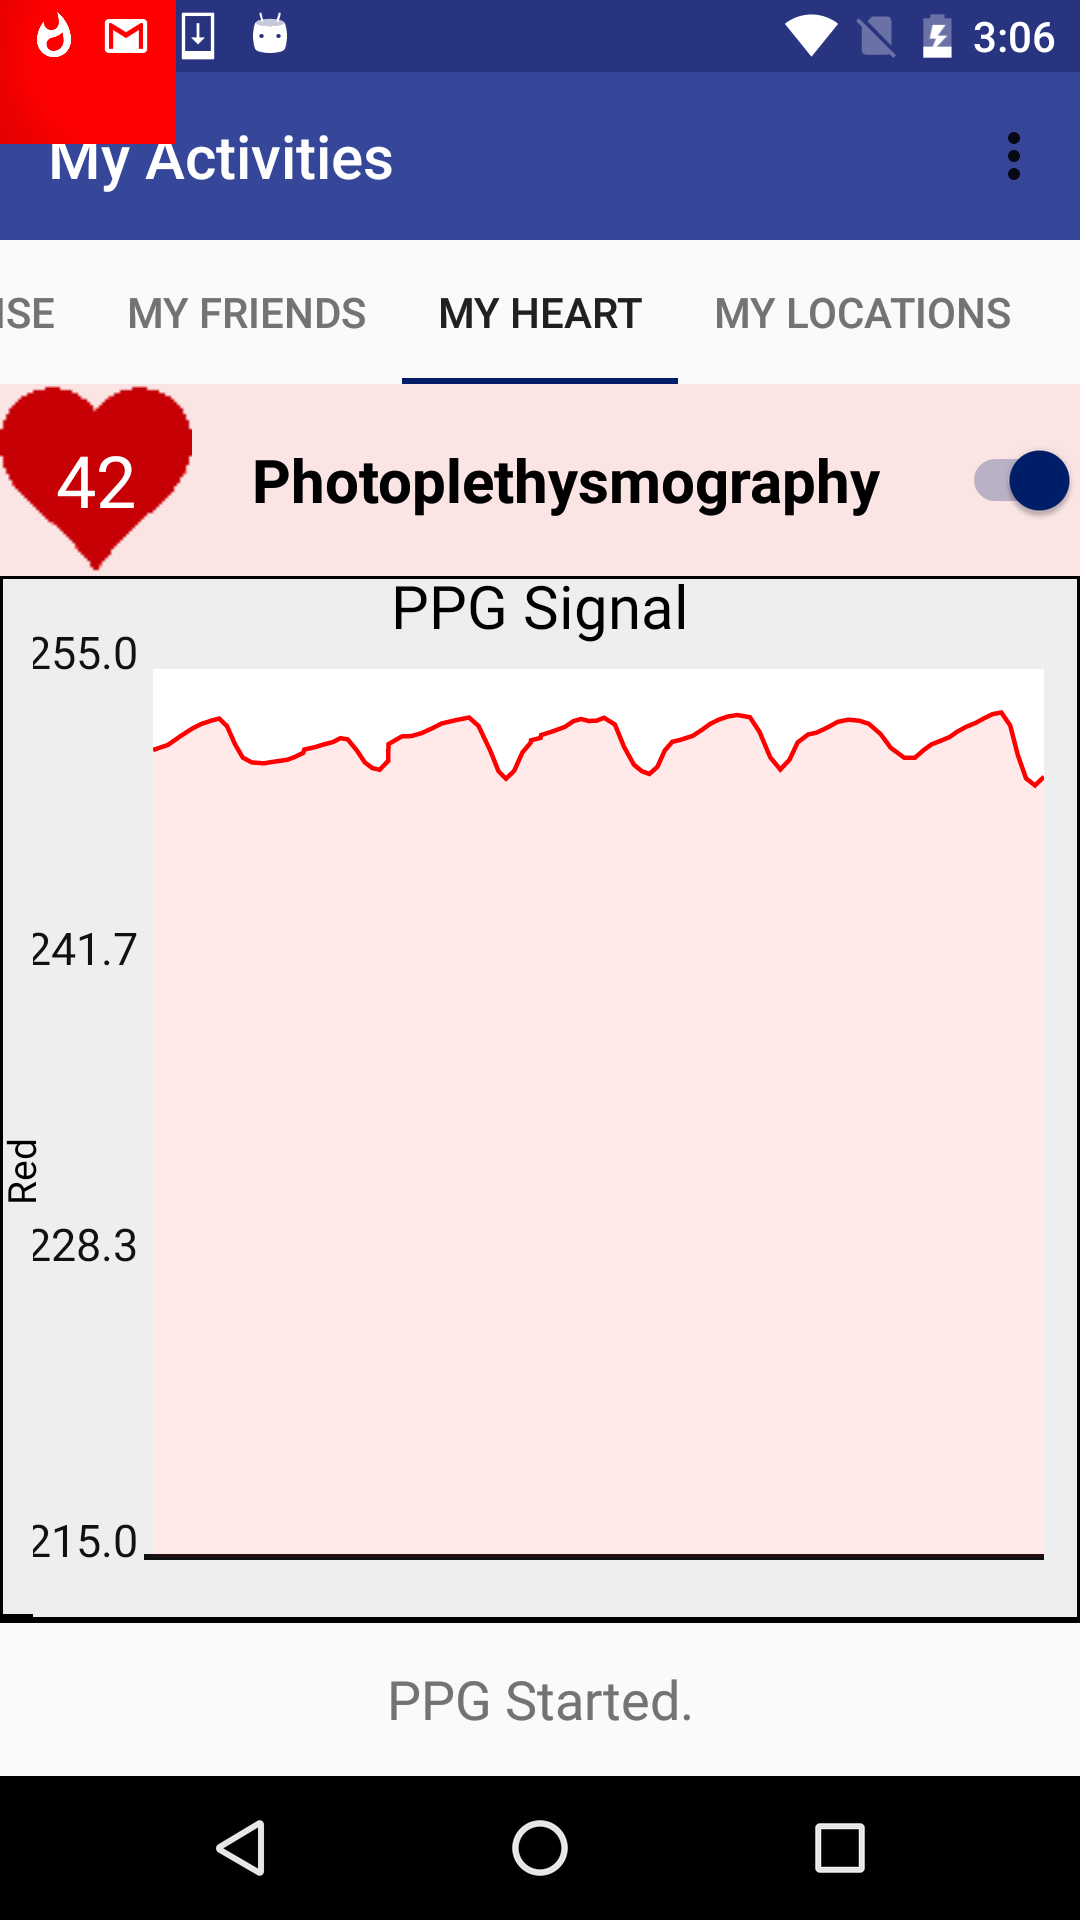
\includegraphics[width=0.402\textwidth]{smoothed_ppg}}
  \quad\quad
  \subfloat[Unsmoothed PPG Signal]{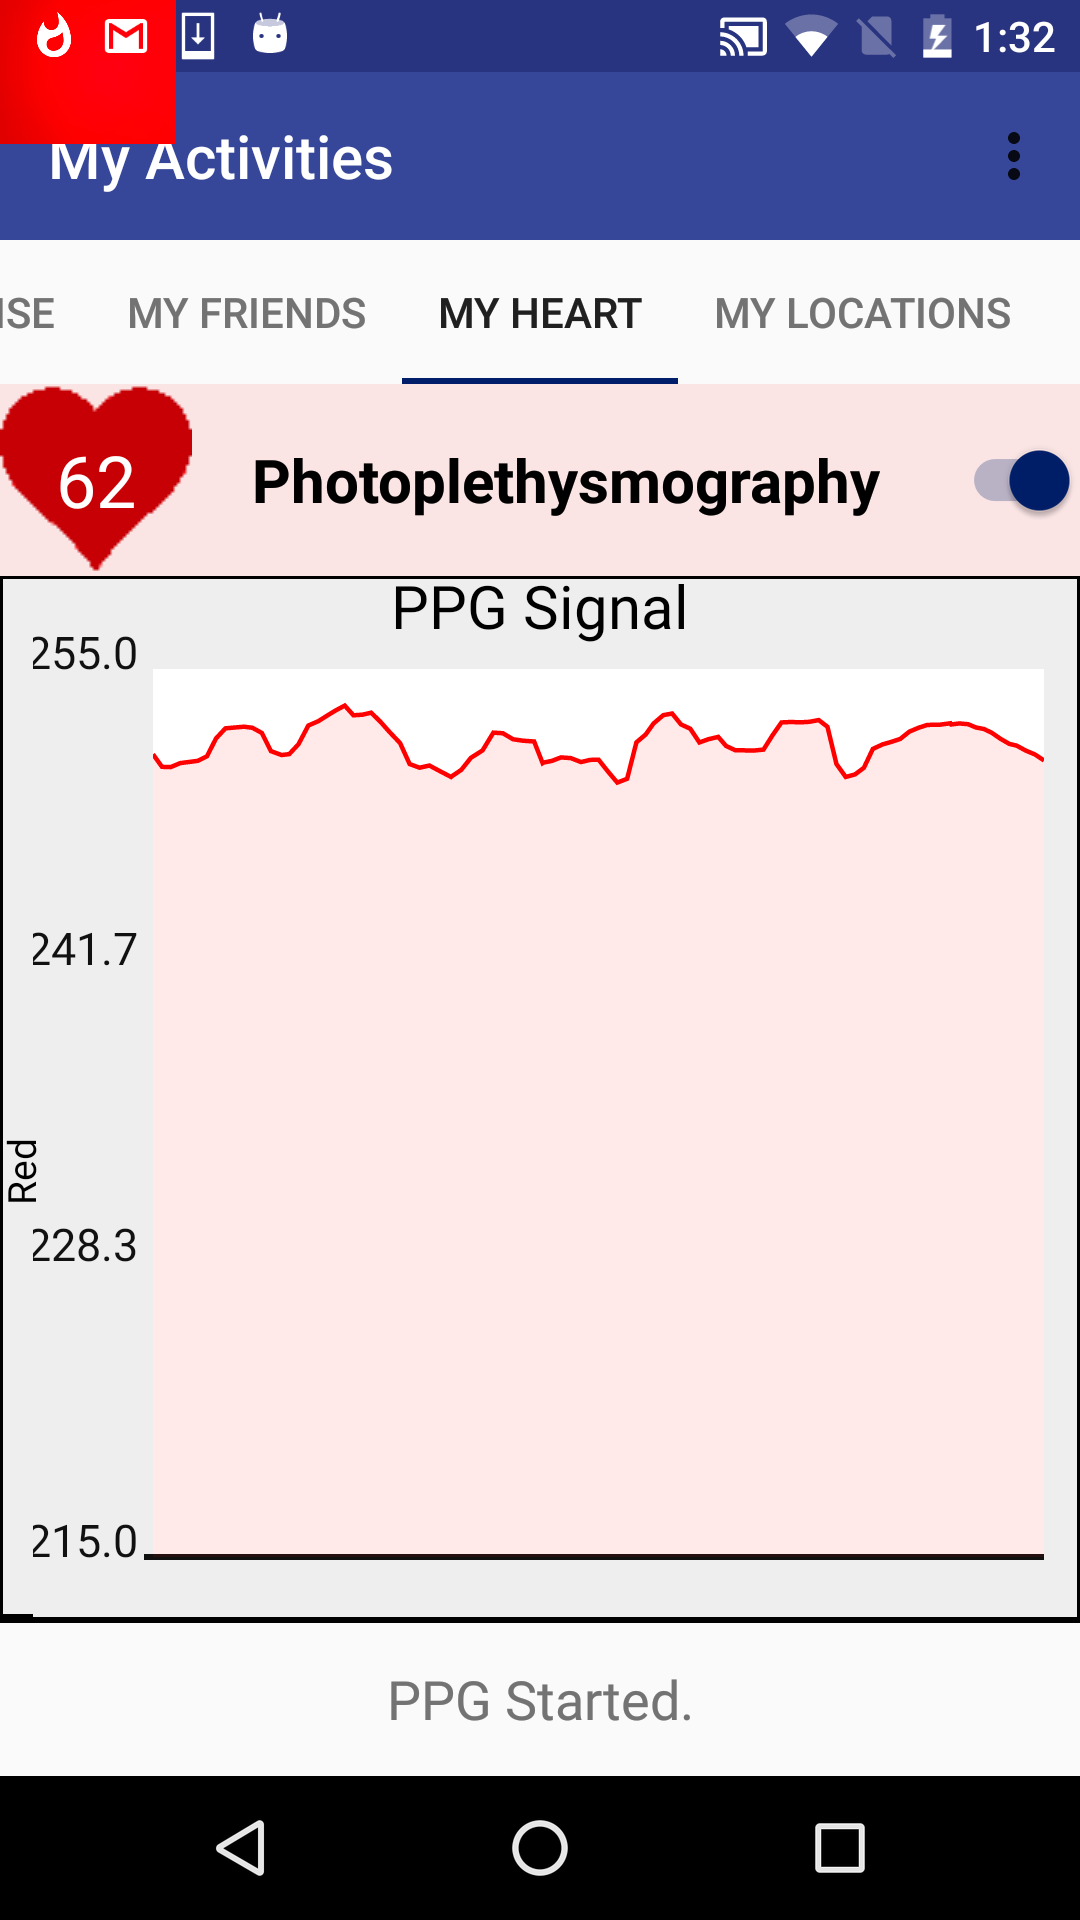
\includegraphics[width=0.402\textwidth]{unsmoothed_ppg}}
  \caption{Smoothed and Unsmoothed PPG Signals}
\end{figure}




% --------------------------------------------------------------
%                         Heart-Rate
% --------------------------------------------------------------
\item \textbf{PPG Signal on Visualization.html}
\begin{enumerate}

\item \textbf{Stationary}
\begin{figure}[!htb]
  \centering
  \subfloat{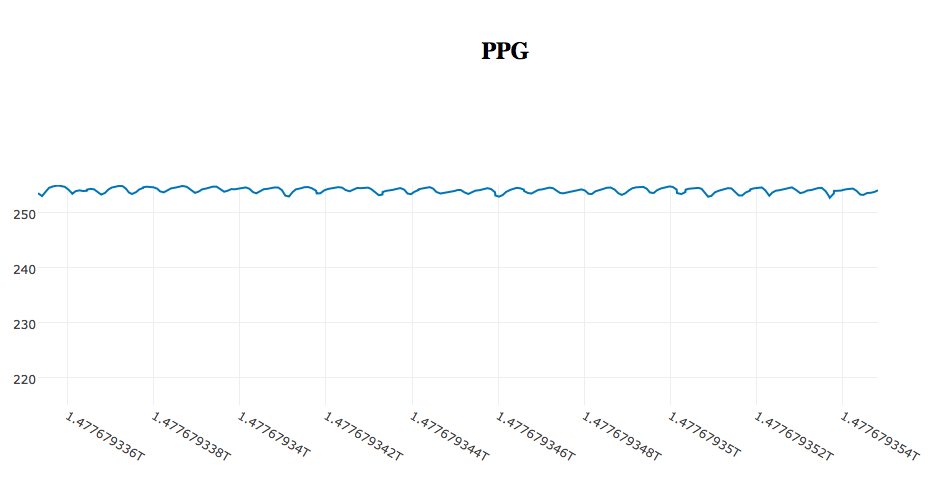
\includegraphics[width=0.90\textwidth]{sedentary_ppg}}
  \caption{Sedentary PPG}
\end{figure}
\vspace{5mm}


\item \textbf{After Vigorous Exercise}
\begin{figure}[!htb]
  \centering
  \subfloat{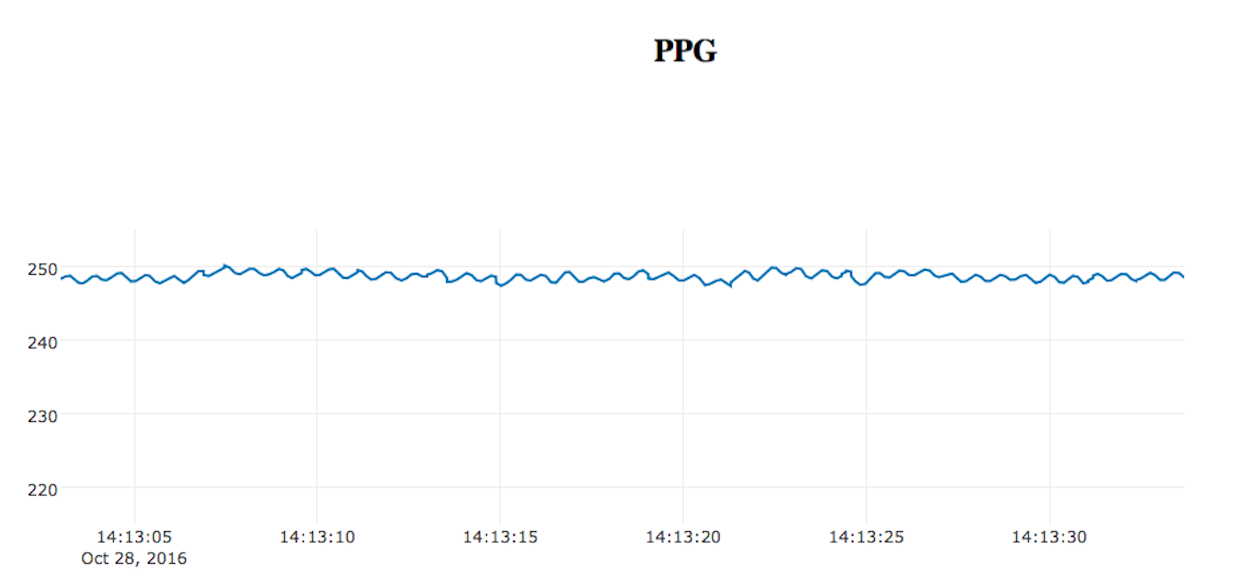
\includegraphics[width=0.93\textwidth]{active_ppg}}
  \caption{Jumping Jacks PPG}
\end{figure}


\end{enumerate}

\newpage
% --------------------------------------------------------------
%                         Computing HRV
% --------------------------------------------------------------
\item \textbf{Computing HRV}

\vspace{4mm}
Heart-rate variability (HRV), the changes in the beat-to-beat heart rate, is an indicator of an individual's cardiovascular condition. HRV has been shown to predict heart attack-related death, depression and congestive heart failure. Heart rate variability can be calculated by taking the standard deviation of the time intervals between beats. To compute it on our phones, we could take the difference between successive timestamps of detected heartbeats, then compute the standard deviation of these differences. 

\vspace{4mm}
We implemented this for the HRV Estimation extra credit.

\vspace{6mm}
\textbf{Source}
\begin{itemize}
\item Huang, R., \& Dung, L. (2016, January 29). Measurement of heart rate variability using off-the-shelf smart phones. \textit{BioMedical Engineering Online.}
\end{itemize}


\vspace{12mm}

\item \textbf{Member Roles \& Contributions}
\begin{itemize}
\item Thai: extracted PPG signal from camera frames, sent sensor readings to server and UI, helped implement heart-rate detection algorithm
\item Susie: chose smoothing parameters, smoothed PPG signal, took screenshots of UI and visualization page, completed report
\item Colin: helped implement heart-rate detection algorithm, implemented HRV \newline computation for extra credit
\end{itemize}




% --------------------------------------------------------------
%     You don't have to mess with anything below this line.
% --------------------------------------------------------------
\end{enumerate}

 
\end{document}